%%%%%%%%%%%%%%%%%%%%%%%%%%%%%%%%%%%%%%%%%%%%%%%%%%%%%%%%%%%%%%%%%%%%%%%%%%%%%%%%%%%%%%%%%%%%%%%%%%%%%%%%%%%%%%%%%%%%%%%%%%%%%%%%%%%%%%%%%%%%%%%%%%%%%%%%%%%%%%%%%%%
% Written By Michael Brodskiy
% Class: Fundamentals of Linear Systems
% Professor: I. Salama
%%%%%%%%%%%%%%%%%%%%%%%%%%%%%%%%%%%%%%%%%%%%%%%%%%%%%%%%%%%%%%%%%%%%%%%%%%%%%%%%%%%%%%%%%%%%%%%%%%%%%%%%%%%%%%%%%%%%%%%%%%%%%%%%%%%%%%%%%%%%%%%%%%%%%%%%%%%%%%%%%%%

\include{Includes.tex}

\title{Homework 4}
\date{\today}
\author{Michael Brodskiy\\ \small Professor: I. Salama}

\begin{document}

\maketitle

\begin{enumerate}

  \item

    \begin{enumerate}

      \item We begin by taking the Laplace transform to get:

        $$H(s)=-\frac{1}{s-1}\quad\text{ and }\quad X(s)=\frac{2}{s}\left[  e^{-s}-e^{-2s}\right]$$

        We then multiply the two to get:

        $$Y(s)=X(s)H(s)$$
        $$Y(s)=-\frac{2}{s(s-1)}\left[ e^{-s}-e^{-2s} \right]$$

        Using partial fraction decomposition, we may write the equivalent such that:

        $$-\frac{2}{s(s-1)}=\frac{A}{s-1}+\frac{B}{s}=As+B(s-1)$$

        We use $s=0,1$ to get:

        $$A=-2,\,B=2\to -\frac{2}{s-1}+\frac{2}{s}$$

        We now distribute this in the above case to get:

        $$Y(s)=-\frac{2}{s-1}\left[ e^{-s}-e^{-2s} \right]+\frac{2}{s}\left[ e^{-s}-e^{-2s} \right]$$
        $$Y(s)=-\frac{2e^{-s}}{s-1}+\frac{2e^{-2s}}{s-1}+\frac{2e^{-s}}{s}-\frac{2e^{-2s}}{s}$$

        Finally, we take the inverse transform to get:

        $$\boxed{y(t)=-2u(1-t)+2e^{t-1}u(1-t)+2u(2-t)-2e^{t-2}u(2-t)}$$

      \item 

        Differentiating one of the inputs is the same as differentiating the output. Thus, we may say:

        $$g(t)=\frac{d}{dt}[y(t)]$$
        $$\boxed{g(t)=2e^{t-1}u(1-t)-2e^{t-2}u(2-t)}$$

      \item As stated in (b) \underline{$g(t)=(d/dt)[y(t)]$}

      \item $z(t)$ is the same as $g(t)$. Since taking the differential is a linear operation, it does not matter if this is done to the impulse response or to $x(t)$. Therefore, we get:

      \item By linearity of the transform, we may say:

        $$y_1(t)=2y(t-1)$$

        Therefore, we may obtain:

        $$\boxed{y_1(t)=-4u(2-t)+4e^{t-2}u(2-t)+4u(3-t)-4e^{t-3}u(3-t)}$$

    \end{enumerate}

  \item

    \begin{enumerate}

      \item We may write the convolution integral as:

        $$y(t)=\int_{-\infty}^{\infty} x(\tau)h(t-\tau)\,d\tau$$

        Expressing this in terms of the provided functions, we may write:

        $$y(t)=\int_{0}^{\infty} e^{-2\tau}e^{\tau-t}\,d\tau$$
        $$y(t)=\int_{0}^{\infty} e^{-(\tau+t)}\,d\tau$$

        Integrating, we obtain:

        $$y(t)= -e^{-(\tau+t)}\Big|_{0}^{\infty}$$
        $$y(t)= -\frac{1}{e^{\infty+t}}-\left( -e^{-t} \right)$$

        Finally, we get (notice the step function returns to set boundaries):

        $$\boxed{y(t)=e^{-t}u(t)}$$

      \item From the provided information for $x(t)$, we see that $x(t)\neq0$ only for $0\leq t\leq 4$. We can then set up the convolution integral as:

        $$y(t)=\int_{-\infty}^{\infty} [u(\tau)-2u(\tau-1)+u(\tau-4)](e^{t-\tau}u(1-t+\tau))\,d\tau$$

        Here, we see that the term provided by $h(t)$ exists only for $\tau\leq t-1$. Thus, we may write:

        $$y(t)=\int_{0}^{t-1} e^{-\tau+t}\,d\tau-2\int_{1}^{t-1} e^{-\tau+t}\,d\tau+\int_{4}^{t-1} e^{-\tau+t}\,d\tau$$

        We evaluate to get:

        $$y(t)=e^t\left[-e^{-\tau}\Big|_0^{t-1}+2e^{-\tau}\Big|_{1}^{t-1}-e^{-\tau}\Big|_4^{t-1}\right]$$
        $$y(t)=e^t\left[(-e^{1-t}+1)+2\left( e^{1-t}-\frac{1}{e} \right)-\left(e^{1-t}-\frac{1}{e^4}\right)\right]$$
        $$y(t)=-e+e^t+2e-e^{t-1}-e+e^{t-4}$$

        And finally, this gets us:

        $$\boxed{y(t)=e^t-e^{t-1}+e^{t-4}}$$

      \item We may break the overlap into cases to evaluate the impulse response. We know that $h(t-\tau)$ extends from $t-2$ to $t-1$, while $x(\tau)$ extends from $0$ to $1$. Thus, we may analyze:

        \begin{itemize}

          \item $t-1 <0$ — There is no overlap

          \item $0<t-1<1$ — There is overlap

          \item $0<t-2<1$ — There is overlap

          \item $t-2>1$ — There is no overlap

        \end{itemize}

        Thus, we may solve for the impulse response using:

        $$y(t)=\int_{-\infty}^{\infty} x(\tau)h(t-\tau)\,d\tau$$
        $$y_1(t)=\int_{0}^{t-1} \sin(\pi \tau)\,d\tau$$
        $$y_2(t)=\int_{t-2}^{1} \sin(\pi\tau)\,d\tau$$
        
        Evaluating, we obtain:

        $$y_1(t)= -\frac{1}{\pi}\left[\cos(\pi \tau)\Big|_0^{t-1}\right]$$
        $$y_2(t)=-\frac{1}{\pi}\left[\cos(\pi\tau)\Big|_{t-2}^1\right]$$
        $$y_1(t)= -\frac{1}{\pi}\left[(\cos(\pi t-\pi)-1)\right]$$
        $$y_2(t)= -\frac{1}{\pi}\left[(-1-\cos(\pi t-2\pi))\right]$$

        Finally, we get:
        
        $$y_1(t)= \frac{1}{\pi}-\frac{\cos(\pi t-\pi)}{\pi}$$
        $$y_2(t)= \frac{1}{\pi}+\frac{\cos(\pi t-2\pi)}{\pi}$$

        Implementing boundaries from the two cases, we write:

        $$y(t)=\left\{\begin{array}{ll} 0, & t-1<0\\\frac{1}{\pi}-\frac{\cos(\pi t-\pi)}{\pi}, & 0<t-1<1\\\frac{1}{\pi}+\frac{\cos(\pi t-2\pi)}{\pi}, & 0<t-2<1\\ 0, & t-2>1\end{array}$$

        This can be simplified as:

        $$\boxed{y(t)=\left\{\begin{array}{ll} 0, & t<1\\\frac{1}{\pi}-\frac{\cos(\pi t-\pi)}{\pi}, & 1<t<2\\\frac{1}{\pi}+\frac{\cos(\pi t-2\pi)}{\pi}, & 2<t<3\\ 0, & t>3\end{array}}$$

      \item 

        We know that the step response can be defined as the integral with respect to time of the impulse response. Assuming zero-state initial conditions, we may write:

        $$s(t)=\int y(t)\,dt$$

        Evaluating the integral, we get:

        $$\boxed{s(t)=\left\{\begin{array}{ll} 0, & t<1\\\frac{t}{\pi}-\frac{\sin(\pi t-\pi)}{\pi^2}, & 1<t<2\\\frac{t}{\pi}+\frac{\sin(\pi t-2\pi)}{\pi^2}, & 2<t<3\\ 0, & t>3\end{array}}$$

    \end{enumerate}

  \item

    \begin{enumerate}

      \item 

        Given the set up, we may write:

        $$\left( \frac{1}{4} \right)^nu[n]-A\left( \frac{1}{4} \right)^{n-1}u[n-1]=\delta[n]$$

        We may redefine the delta as:

        $$\left( \frac{1}{4} \right)^nu[n]-A\left( \frac{1}{4} \right)^{n-1}u[n-1]=u[n]-u[n-1]$$

        Thus, we see that we need the exponential term to cancel. We can do this by simply taking:

        $$\left( \frac{1}{4} \right)^n=A\left( \frac{1}{4} \right)^{n-1}$$

        Dividing the exponential from one side to the other, we see:

        $$A=\left( \frac{1}{4} \right)^1$$
        $$\boxed{A=\frac{1}{4}}$$

      \item 

        By definition, with $h[n]$ and $g[n]=h_{inv}[n]$, we know:

        $$h[n]*g[n]=\delta[n]$$

        Using the equation from part (a), we know:

        $$h[n]-Ah[n-1]=\delta[n]$$

        By the properties of convolution, we know that:

        $$x[n]*\delta[n-n_o]=x[n-n_o]$$

        Thus, we may expand to write:

        $$h[n]*\delta[n]-Ah[n]*\delta[n-1]=\delta[n]$$
        $$h[n]*(\delta[n]-A\delta[n-1])=\delta[n]$$

        Thus, combining this with the definition of inverse, we may write:

        $$\boxed{g[n]=\delta[n]-\frac{1}{4}\delta[n-1]}$$

      \item To find the step response from the impulse response, we may simply sum with respect to $n$:

        $$s[n]=\sum_{k=0}^{\infty} \left( \frac{1}{4} \right)^{n-k}u[n]$$

        By our series simplification formulas, we may write:

        $$s[n]=\frac{1-\left( \frac{1}{4} \right)^{n+1}}{1-.25}u[n]$$
        $$\boxed{s[n]=\left[4-\left( \frac{1}{4} \right)^{n}\right]u[n]}$$

    \end{enumerate}

  \item

    \begin{enumerate}

      \item We may observe that the system is \underline{not causal}, since it is non-zero for $n<0$. Expressing the sum, we may see that:

        $$\sum_{-\infty}^3 3^nu[3-n]\text{ is finite}$$

        And, therefore, the system \underline{is stable}

      \item We may see that, for $n<0$, the system is zero, and, therefore, the system \underline{is causal}. We can break the system apart to analyze stability:

        $$\sum_0^{\infty} \left( \frac{1}{2} \right)^n + \sum_{3}^{\infty} (1.1)^n$$

        We may see that, though the first term is finite, the second term is not. Therefore, the system is \underline{not stable}.

      \item We may see that, due to the $u[2-n]$ term, there are values $n<0$ for which the function is non-zero, meaning it is \underline{not causal}. In terms of stability, we may write (taking the effect of $\cos$ as worst case magnitude, or 1):

        $$\sum_{0}^{\infty}\left( \frac{1}{2} \right)^n+\sum_{-\infty}^2 (1.1)^n$$

        We may thus see that both terms are bounded, and, therefore, the system is \underline{stable}.

      \item We may see that, for $n<0$ the system is zero; therefore, the system \underline{is causal}. Analyzing stability, we see:

        $$\sum_0^{\infty} n\left( \frac{1}{3} \right)^n$$
        $$\sum_0^{\infty} n(3)^{-n}\text{ is finite}$$

        Thus, the system \underline{is stable}

    \end{enumerate}

  \item

    \begin{enumerate}

      \item For the given system, we may see that, for $t<0$, the response may be non-zero (more precisely, it is non-zero for $-\infty< t<5$); therefore, the system is \underline{not causal}. We check for stability below:

        $$\int_{-\infty}^{5}e^{-3t}\,dt$$
        $$-\frac{e^{-3t}}{3}\Big|_{-\infty}^5=\infty$$

        Therefore, the system is \underline{not stable}

      \item We may see that, for the given system, for $t<0$, the response may be non-zero (more precisely, it is non-zero for $t>-10$); therefore, the system is \underline{not causal}. We check for stability below:

        $$\int_{-10}^{\infty}e^{-4t}\,dt$$
        $$-\frac{e^{-4t}}{4}\Big_{-10}^{\infty}=\frac{e^{40}}{4}<\infty$$

        Thus, we see that the system is \underline{stable}

      \item 

        We may rewrite the function as:

        $$x(t)=\left\{\begin{array}{ll} e^{-2t}, & t\geq0\\ e^{2t}, & t<0\end{array}$$

        Because the value of the function is non-zero when $t<0$, we can see that it is \underline{not causal}

        We may check for stability below:

        $$\int_{-\infty}^{0} e^{2t}\,dt + \int_0^{\infty} e^{-2t}\,dt$$
        $$\frac{e^{2t}}{2}\Big|_{-\infty}^0-\frac{e^{-2t}}{2}\Big|_0^{\infty}=1$$

        Therefore, we may see that the system is \underline{stable}

      \item We may see that, because the system is zero for $t\leq 0$, it \underline{is causal}. We now check for stability:

        $$\int_2^{\infty} 3e^{-2t}-e^{-.05t+5}\,dt$$
        $$3e^{-2t}-e^{-.05t+5}\Big|_2^{\infty}=e^{4.9}-\frac{3}{e^4}<\infty$$

        Therefore, we may see that the system is \underline{stable}

    \end{enumerate}

  \item

    We may begin by observing that $x(t)$ may be expressed as a summation of impulses, written as:

    $$x(t)=\sum_{n=-\infty}^{\infty} \delta(t-nT)$$

    Convolving this with $h(t)$, by the property that $x(t)*\delta(t-t_o)=x(t-t_o)$, we may write:

    $$y(t)=\sum_{n=-\infty}^{\infty} h(t-nT)$$

    To expand this, we may write:

    $$y(t)=\cdots+h(t+3T)+h(t+2T)+h(t+T)+h(t)+h(t-T)+h(t-2T)+h(t-3T)+\cdots$$

    We begin by analyzing the $T=1$ case. Summing these graphically, we obtain:

    \begin{figure}[H]
      \centering
      \tikzset{every picture/.style={line width=0.75pt}} %set default line width to 0.75pt        

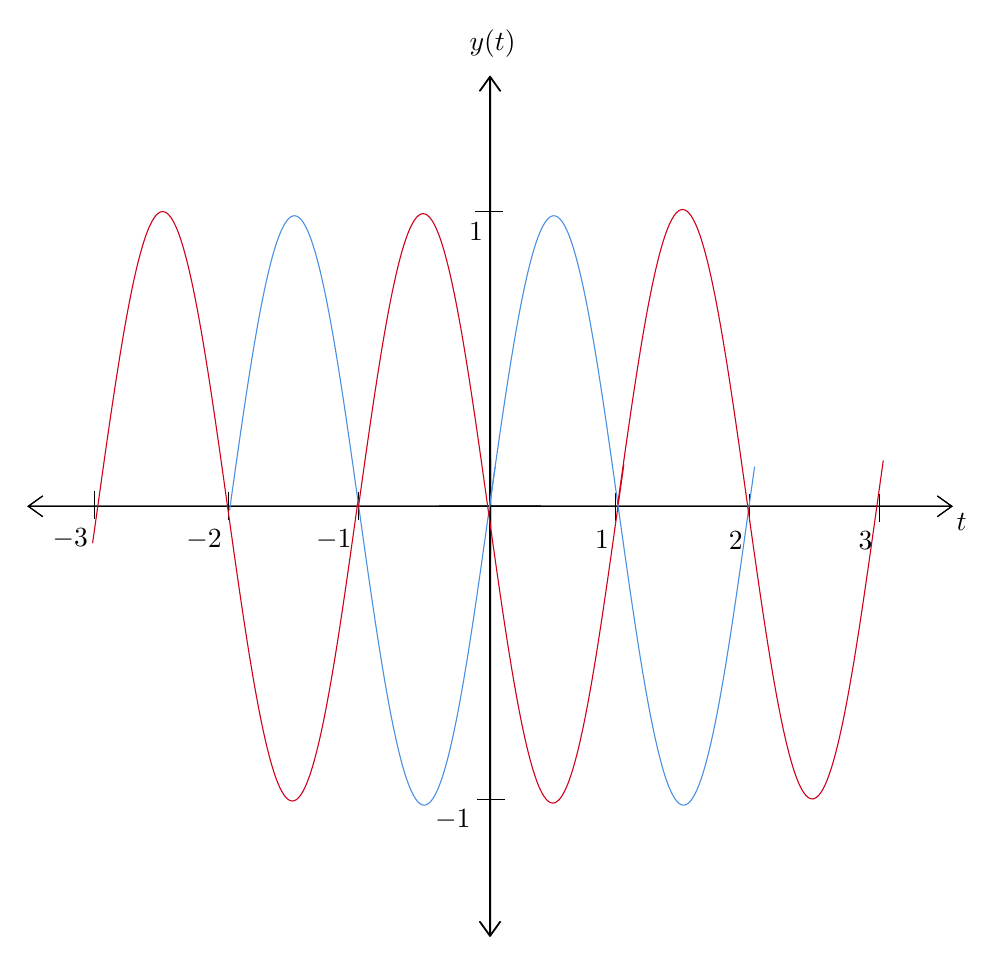
\begin{tikzpicture}[x=0.75pt,y=0.75pt,yscale=-1,xscale=1]
%uncomment if require: \path (0,474); %set diagram left start at 0, and has height of 474

%Shape: Axis 2D [id:dp7161537544794797] 
\draw  (244,268) -- (491,268)(268.7,61) -- (268.7,291) (484,263) -- (491,268) -- (484,273) (263.7,68) -- (268.7,61) -- (273.7,68)  ;
%Shape: Axis 2D [id:dp28833393699455456] 
\draw  (244,268) -- (491,268)(268.7,475) -- (268.7,245) (484,273) -- (491,268) -- (484,263) (263.7,468) -- (268.7,475) -- (273.7,468)  ;
%Shape: Axis 2D [id:dp347226092427816] 
\draw  (293,268) -- (46,268)(268.3,61) -- (268.3,291) (53,263) -- (46,268) -- (53,273) (273.3,68) -- (268.3,61) -- (263.3,68)  ;
%Shape: Axis 2D [id:dp4308838695209243] 
\draw  (293,268) -- (46,268)(268.3,475) -- (268.3,245) (53,273) -- (46,268) -- (53,263) (273.3,468) -- (268.3,475) -- (263.3,468)  ;
%Straight Lines [id:da576607479960361] 
\draw    (274.71,126) -- (261.29,126) ;
%Straight Lines [id:da8477926380861857] 
\draw    (275.72,409.42) -- (262.3,409.42) ;
%Straight Lines [id:da6838520777567837] 
\draw    (329.01,275.13) -- (329.01,261.71) ;
%Straight Lines [id:da6857013828052266] 
\draw    (393.54,275.42) -- (393.54,262) ;
%Straight Lines [id:da9256429599572711] 
\draw    (455.96,275.42) -- (455.96,262) ;
%Straight Lines [id:da8842959666301083] 
\draw    (78.01,274.13) -- (78.01,260.71) ;
%Straight Lines [id:da011159065569899873] 
\draw    (142.54,274.42) -- (142.54,261) ;
%Straight Lines [id:da9631744630520165] 
\draw    (204.96,274.42) -- (204.96,261) ;
%Shape: Wave [id:dp22801073904152536] 
\draw  [color={rgb, 255:red, 208; green, 2; blue, 27 }  ,draw opacity=1 ] (77.01,285.79) .. controls (77.84,279.91) and (78.67,273.97) .. (79.51,268) .. controls (89.7,195.26) and (99.45,126) .. (110.76,126) .. controls (122.07,126) and (131.82,195.26) .. (142.01,268) .. controls (152.2,340.74) and (161.95,410) .. (173.26,410) .. controls (184.57,410) and (194.32,340.74) .. (204.51,268) .. controls (204.66,266.92) and (204.81,265.84) .. (204.96,264.76) ;
%Shape: Wave [id:dp6897913338521096] 
\draw  [color={rgb, 255:red, 74; green, 144; blue, 226 }  ,draw opacity=1 ] (143,270) .. controls (153.19,197.26) and (162.94,128) .. (174.25,128) .. controls (185.56,128) and (195.31,197.26) .. (205.5,270) .. controls (215.69,342.74) and (225.44,412) .. (236.75,412) .. controls (248.06,412) and (257.81,342.74) .. (268,270) .. controls (268.99,262.92) and (269.98,255.88) .. (270.96,248.93) ;
%Shape: Wave [id:dp5735373017928471] 
\draw  [color={rgb, 255:red, 208; green, 2; blue, 27 }  ,draw opacity=1 ] (205,269) .. controls (215.19,196.26) and (224.94,127) .. (236.25,127) .. controls (247.56,127) and (257.31,196.26) .. (267.5,269) .. controls (277.69,341.74) and (287.44,411) .. (298.75,411) .. controls (310.06,411) and (319.81,341.74) .. (330,269) .. controls (330.99,261.92) and (331.98,254.88) .. (332.96,247.93) ;
%Shape: Wave [id:dp04377834135397385] 
\draw  [color={rgb, 255:red, 74; green, 144; blue, 226 }  ,draw opacity=1 ] (268,270) .. controls (278.19,197.26) and (287.94,128) .. (299.25,128) .. controls (310.56,128) and (320.31,197.26) .. (330.5,270) .. controls (340.69,342.74) and (350.44,412) .. (361.75,412) .. controls (373.06,412) and (382.81,342.74) .. (393,270) .. controls (393.99,262.92) and (394.98,255.88) .. (395.96,248.93) ;
%Shape: Wave [id:dp5492419839564252] 
\draw  [color={rgb, 255:red, 208; green, 2; blue, 27 }  ,draw opacity=1 ] (330,267) .. controls (340.19,194.26) and (349.94,125) .. (361.25,125) .. controls (372.56,125) and (382.31,194.26) .. (392.5,267) .. controls (402.69,339.74) and (412.44,409) .. (423.75,409) .. controls (435.06,409) and (444.81,339.74) .. (455,267) .. controls (455.99,259.92) and (456.98,252.88) .. (457.96,245.93) ;

% Text Node
\draw (266.3,129.98) node [anchor=north east] [inner sep=0.75pt]    {$1$};
% Text Node
\draw (260.3,412.82) node [anchor=north east] [inner sep=0.75pt]    {$-1$};
% Text Node
\draw (327.01,278.53) node [anchor=north east] [inner sep=0.75pt]    {$1$};
% Text Node
\draw (391.54,278.82) node [anchor=north east] [inner sep=0.75pt]    {$2$};
% Text Node
\draw (453.96,278.82) node [anchor=north east] [inner sep=0.75pt]    {$3$};
% Text Node
\draw (202.96,277.82) node [anchor=north east] [inner sep=0.75pt]    {$-1$};
% Text Node
\draw (140.54,277.82) node [anchor=north east] [inner sep=0.75pt]    {$-2$};
% Text Node
\draw (76.01,277.53) node [anchor=north east] [inner sep=0.75pt]    {$-3$};
% Text Node
\draw (269.72,53) node [anchor=south] [inner sep=0.75pt]    {$y( t)$};
% Text Node
\draw (492,270.4) node [anchor=north west][inner sep=0.75pt]    {$t$};


\end{tikzpicture}

      \caption{$T=1$ Case Graphically Summed}
      \label{fig:1}
    \end{figure}

    For ease of interpretation, the graph above shows the sum expanded above, with $n$ even cases in red and $n$ odd in blue. We may thus see that, summing the two, we simply obtain $\boxed{y(t)=0\Big|_{T=1}}$, or a flat line on the $t$ axis. Applying similar logic to $T=2$, we may draw the corresponding sinusoids to find:

    \begin{figure}[H]
      \centering
      \include{Figures/HW4-6b}
      \caption{$T=2$ Case Graphically Summed}
      \label{fig:2}
    \end{figure}

    We may observe that this sinusoid consists solely of the even sinusoids from Figure \ref{fig:1}. This makes sense, as using $T=2$ effectively doubles every $n$, making the shift even. Therefore, we obtain the solution shown in Figure \ref{fig:2}. We may write this as:

    $$y(t)=\cdots+h(t+6)+h(t+4)+h(t+2)+h(t)+h(t-2)+h(t-4)+h(t-6)+\cdots$$
    $$\boxed{y(t)=\sum_{n=-\infty}^{\infty} h(t-2n)}$$

  \item

    \begin{enumerate}

      \item Given the form of $x(t)$, we know $y(t)$ is of the form:

        $$y(t)=Ae^{(-1+2j)t}$$

        Plugging this into the given equation, we get:

        $$A(-1+2j)e^{(-1+2j)t}+3Ae^{(-1+2j)t}=e^{(-1+2j)t}$$

        This simplifies to:

        $$A(-1+2j)+3A=1$$
        $$A=\frac{1}{2j+2}$$

        And gives us the particular equation:

        $$y_p(t)=\frac{e^{(-1+2j)t}}{2j+2}$$

        We can now find the homogenous solution, with general form of $y(t)$:

        $$y_h(t)=Ae^{\lambda t}$$

        Using our equation, we may obtain:

        $$A\lambda e^{\lambda t}+3Ae^{\lambda t}=0$$
        $$\lambda=-3$$

        Combing the two we get:

        $$y(t)=Ae^{-3 t}+\frac{e^{(-1+2j)t}}{2j+2}$$

        Applying the initial rest condition, we get:

        $$0=A+\frac{1}{2j+2}$$
        $$A=-\frac{1}{2j+2}$$

        Thus, ensuring that there is a response only for $t>0$, we finally get:

        $$\boxed{y(t)=\frac{1}{2+2j}\left[ e^{(-1+2j)t}-e^{-3t} \right]u(t)}$$

      \item 

        We can expand our answer from (a):

        $$y(t)=\frac{1}{2+2j}\left[ e^{-t}\cos(2t)+je^{-t}\sin(2t)-e^{-3t} \right]u(t)$$

        Multiplying by the conjugate, we get:

        $$y(t)=(.25-.25j)\left[ e^{-t}\cos(2t)+je^{-t}\sin(2t)-e^{-3t} \right]u(t)$$
        $$y(t)=\left[ .25e^{-t}\cos(2t)+.25e^{-t}\sin(2t)-.25e^{-3t} \right]u(t)$$

        Therefore, our output becomes:

        $$\boxed{y(t)=\left[ .25e^{-t}\sin(2t)+.25e^{-t}\cos(2t)-.25e^{-3t}\right]u(t)}$$

    \end{enumerate}

  \item

    \begin{itemize}

      \item We know that the equations governing time response of an inductor and capacitor are (respectively):

        $$y(t)=L\frac{di(t)}{dt}\quad\text{ and }i(t)=C\frac{dV_c(t)}{dt}$$

        We know that the voltage across the capacitor will be the difference between the voltage supplied and the voltage across the inductor; thus, we may write:

        $$i(t)=C\frac{d}{dt}\left[ x(t)-y(t) \right]$$

        Inserting this into the inductor equation, we get:

        $$y(t)=L\frac{d}{dt}\left[ C\frac{d}{dt}\left[ x(t)-y(t) \right] \right]$$
        $$y(t)=LC\frac{d^2}{dt^2}\left[x(t)-y(t) \right]$$

        Putting similar terms to one side, we may write:

        $$\frac{d^2y(t)}{dt^2}+\frac{1}{LC}y(t)=\frac{d^2x(t)}{dt^2}$$

        Inserting known values:

        $$\boxed{\frac{d^2y(t)}{dt^2}+25y(t)=\frac{d^2x(t)}{dt^2}}$$

      \item 

        Taking $x(t)\to0$, we find the homogenous solution form as:

        $$\frac{d^2y(t)}{dt^2}+25y(t)=0$$

        Using the provided equation, we insert into the above:

        $$\left[ K_1\omega_1^2e^{j\omega_1 t}+K_2\omega_2^2e^{j\omega_2t} \right]+25\left[ K_1e^{j\omega_1 t}+K_2e^{j\omega_2t} \right]=0$$

        Dividing by the exponentials, we get:

        $$K_1\omega_1^2+K_2\omega_2^2+25K_1+25K_2=0$$

        By observation, we may see that:

        $$\boxed{\omega_1=\omega_2=\pm5}$$

      \item 

        From part (b), we see that the natural (homogenous) response may be modeled by:

        $$y(t)=Ae^{j5t}+Be^{-j5t}$$

        We may take $A=\frac{1}{2}(a+b)$ and $B=\frac{1}{2}(a-b)$. We then apply Euler's Law to get:

        $$\boxed{y(t)=a\cos(5t)+b\sin(5t)}$$

        We may thus observe that the natural response is sinusoidal in nature.

    \end{itemize}

\end{enumerate}

\end{document}

